\documentclass[11pt, a4paper]{article}
\usepackage[utf8]{inputenc}
\usepackage{graphicx}
\usepackage{amssymb}
\usepackage{amsmath}
\graphicspath{{figs/}}
\title{AI1110 Assignment 1}
\author{Abhinav Yadav, cs21btech11002}

\begin{document}
    \maketitle
    \section*{Q11 (b)}
    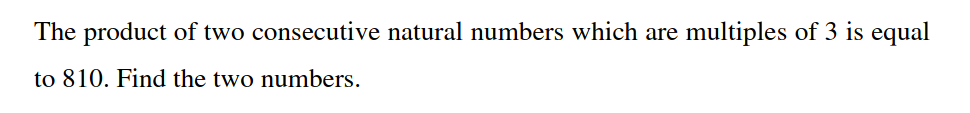
\includegraphics[width=\textwidth]{q11_b.png}
    \section*{Solution}
    Let the two consecutive natural numbers which are multiples of $3$ be $3n$ and $3n+3$
    \hspace{5pt} $\exists \hspace{2pt} n \in \mathbb{N}$\\\\
    \textbf{According to the question:}
    \begin{align*}
        & 3n(3n+3) = 810\\
        \Rightarrow & 9n(n+1)=810\\
        \Rightarrow & n(n+1)=90\\
        \Rightarrow & n^2+n-90=0\hspace{40pt} -(1)\\
        \Rightarrow & (n+10)(n-9)=0\\
        \Rightarrow & n=-10 \hspace{15pt} or \hspace{15pt} n=9
    \end{align*}
    \begin{center}
        discarding $n=-10$ as $n \in \mathbb{N}$
    \end{center}
    \begin{equation*}
        \begin{split}
            \Rightarrow & n=9\\
            \Rightarrow & 3n=27\\
            \Rightarrow & 3n+3=30\\\\
        \end{split}
    \end{equation*} 
    The two numbers are:\\
    \fbox{$27, 30$}\pagebreak

    Plot of $eq^n(1)$ is:\\
    \begin{figure}[h]
        \centering
        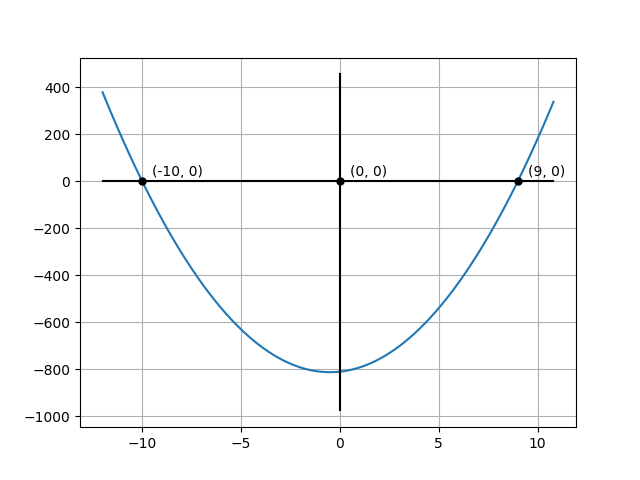
\includegraphics[width=0.8\textwidth]{plot.png}
        \caption{Plot showing the polynomial in $eq^n(1)$}
    \end{figure}\\
    It can be easily verified by observing the plot that the roots of $eq^n (1)$ are 9 and -10.\\\\

    The output of the program used to find and verify these numbers is:
    \begin{figure}[h]
        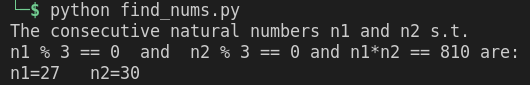
\includegraphics[width=\textwidth]{output.png}
        \caption{Output of the python program}
    \end{figure}
\end{document}